\documentclass[10pt,conference]{IEEEtran}

\usepackage{amsmath}
\usepackage{amssymb}
\usepackage{array}
\usepackage{booktabs}
\usepackage{cite}
\usepackage{graphicx}
\usepackage{microtype}
\usepackage{url}
\usepackage{xcolor}
\usepackage{xspace}

\graphicspath{{generated/}}
\newcommand{\SampleRows}{994,496\xspace}
\newcommand{\PhysicalObservations}{248,624\xspace}
\newcommand{\SampleSessions}{97,248\xspace}
\newcommand{\FinalRows}{897,056\xspace}
\newcommand{\TestRows}{179,328\xspace}
\newcommand{\TestPoorRate}{41.43\%\xspace}
\newcommand{\RFAccuracy}{0.9018\xspace}
\newcommand{\RFPrecision}{0.8860\xspace}
\newcommand{\RFRecall}{0.8755\xspace}
\newcommand{\RFFone}{0.8807\xspace}
\newcommand{\RFPRAUC}{0.9549\xspace}
\newcommand{\RFROCAUC}{0.9637\xspace}
\newcommand{\RFBrier}{0.0715\xspace}
\newcommand{\RFECE}{0.0116\xspace}
\newcommand{\FalsePositives}{8,365\xspace}
\newcommand{\FalseAlarmRate}{7.96\%\xspace}
\newcommand{\MeanLead}{9.649\xspace}
\newcommand{\MedianLead}{9.999\xspace}
\newcommand{\PninetyfiveLead}{13.088\xspace}
\newcommand{\Coverage}{90.40\%\xspace}
\newcommand{\AbstentionRate}{9.60\%\xspace}
\newcommand{\AbstainedCount}{17,212\xspace}
\newcommand{\AcceptedAccuracy}{0.9340\xspace}
\newcommand{\AcceptedPrecision}{0.9299\xspace}
\newcommand{\AcceptedRecall}{0.9091\xspace}
\newcommand{\AcceptedFone}{0.9194\xspace}
\newcommand{\DecisionThreshold}{0.37\xspace}
\newcommand{\TrustThreshold}{0.671185\xspace}


\newcommand{\qoe}{\mathrm{QoE}}
\newcommand{\mos}{\mathrm{MOS}}
\newcommand{\ece}{\mathrm{ECE}}
\newcommand{\pr}{\mathrm{PR\mbox{-}AUC}}
\newcommand{\etal}{\textit{et al.}}

\title{A Calibrated Trace-Driven 5G QoE Digital Twin\\
for Trustworthy Next-Observation Forecasting and Grounded Explanations}

\author{
\IEEEauthorblockN{Mohamed Oussama Bouriga and Ahmed Aziz Ben Aissa}
\IEEEauthorblockA{PGE 5 -- Artificial Intelligence and Data Science\\
Aivancity School for Technology, Business \& Society, Cachan, France}
}

\begin{document}
\maketitle

\begin{abstract}
This paper presents a scientifically scoped, trace-driven Digital
Twin for video-streaming Quality of Experience (QoE) forecasting in 5G New
Radio.  The prototype chronologically replays public 5G-QoERA observations,
maintains network and service state, predicts whether the next observation has
poor QoE, calibrates the resulting probability, and attaches a heuristic trust
indicator with selective abstention.  A persistence baseline and a
network-only Logistic Regression are compared with a cross-layer Random
Forest that combines throughput, location, resource allocation, packet loss,
bitrate, resolution, current Mean Opinion Score (MOS), and past-only temporal
features.  The event is defined explicitly as
$\mos_{t+1}<3.0$; the observed one-step interval has median
\MedianLead~s.  On \TestRows sealed chronological test rows, isotonic
calibration and a validation-selected decision threshold of
\DecisionThreshold yielded F1=\RFFone, PR-AUC=\RFPRAUC,
Brier=\RFBrier, and ECE=\RFECE.  There were \FalsePositives false alarms
(\FalseAlarmRate).  A validation-selected trust threshold abstained on
\AbstentionRate of cases and increased accepted-decision accuracy from
\RFAccuracy to \AcceptedAccuracy at \Coverage coverage.  Finally, a grounded
language-model component verbalizes a restricted evidence object but cannot
change the prediction.  All 30 retained explanations passed strict schema and
deterministic grounding validation; one reviewer marked all 30 factually
correct and complete with no unsupported statements.  The results answer the
research question affirmatively but with important qualifications: strong
classification, low aggregate calibration error, and useful selective
accuracy coexist in this dataset, while generalization, sample provenance,
semantic grounding, and multi-reviewer evidence remain open limitations.
\end{abstract}

\begin{IEEEkeywords}
5G New Radio, Quality of Experience, digital twin, video streaming,
chronological replay, probability calibration, Brier score, selective
prediction, trustworthy artificial intelligence, grounded language model.
\end{IEEEkeywords}

\section{Introduction}

Large populations of connected objects increasingly collect and transport
short video segments through access networks and edge services.  An airport
camera, agricultural sensor, vehicle, or mobile terminal observes only a
small part of a distributed service, yet the final user judges the assembled
experience.  Throughput alone cannot represent that judgment: packet loss,
requested bitrate, resolution, scheduling resources, location, mobility, and
recent QoE interact over time.  A useful management prototype must therefore
represent evolving cross-layer state, anticipate a service event, and report
how much confidence an operator should place in the warning.

The public 5G-QoERA dataset was designed for integrated QoE analysis in 5G NR
and combines user mobility, real base-station deployments, radio-map context,
scheduling decisions, application settings, packet-loss observations, and
MOS labels \cite{boffetti2025qoeira}.  The dataset enables a small but
scientifically valid trace-driven twin: a replay engine can consume recorded
observations in time order, update state as an online service would, and test a
future-event forecast without claiming to be a complete commercial twin.

This study asks: \emph{does a cross-layer model that classifies future poor
QoE accurately also produce probabilities reliable enough for trustworthy
network-management support?}  We operationalize ``trustworthy'' narrowly and
measurably.  The system must preserve chronology, prevent target leakage,
calibrate its best classifier, quantify false alarms and timing, abstain when a
validation-selected reliability score is too low, and reject a language-model
explanation if it invents evidence.

The contributions are:

\begin{itemize}
\item a chronological, session-aware replay state spanning radio/resource,
      mobility, and video-service variables;
\item a one-observation-ahead MOS event and leakage-safe temporal evaluation;
\item the required comparison of persistence, network-only Logistic
      Regression, and cross-layer Random Forest models;
\item validation-only calibration, threshold selection, trust scoring, and
      selective abstention;
\item a schema-constrained, evidence-grounded explanation layer that is
      separated from prediction and control; and
\item a reproducible reporting workflow that regenerates every result in this
      paper from validated experiment artifacts.
\end{itemize}

\section{State of the Art}

\subsection{5G Video QoE Modelling}

QoE estimates the quality perceived by a user, whereas network Quality of
Service describes technical delivery.  For video, identical throughput can
produce different experience under different requested bitrates; packet loss
may have little effect in one operating region and severe effect in another.
The novelty of 5G-QoERA is precisely this integration of mobility, scheduling,
deployment, and application details with MOS \cite{boffetti2025qoeira}.
Many conventional supervised pipelines nevertheless flatten such traces into
independent rows.  That practice overstates operational realism because a
prediction at time $t$ is conditioned by earlier state and because random
splits can expose future operating regimes during training.

\subsection{Trace-Driven Network Digital Twins}

ITU-T Y.3090 specifies requirements and architecture for Digital Twin
Networks \cite{itut2022y3090}.  The broader research literature describes a
network twin as a data-driven representation that supports analysis,
diagnosis, simulation, and management while remaining synchronized with the
physical system \cite{almasan2022dtn}.  The present work implements the
limited offline subset appropriate to an assignment prototype: chronological
trace replay, explicit state, future prediction, and an uncertainty/trust
output.  It does not claim bidirectional synchronization, counterfactual
simulation, or autonomous control.

\subsection{Calibration and Selective Prediction}

A classifier's discrimination and its probability reliability are different
properties.  Guo \etal{} showed why post-hoc calibration must be evaluated
separately from accuracy \cite{guo2017calibration}.  Platt scaling fits a
sigmoid mapping \cite{platt1999probabilistic}; isotonic regression instead
learns a monotonic non-parametric mapping.  Proper scores such as the Brier
score \cite{brier1950verification} penalize probabilistic error, while ECE
summarizes the weighted absolute difference between confidence and empirical
frequency across bins \cite{naeini2015calibration}.  ECE is useful but depends
on binning and should not be interpreted as a guarantee for every individual
case.

Selective classification adds a reject option.  Rather than forcing a
decision for every row, a system can trade coverage for lower risk among
accepted predictions \cite{geifman2017selective,geifman2019selectivenet}.
This is suitable for an operator-support twin: an abstention requests more
evidence or human review, while an accepted forecast can support a bounded
decision.  The trust score used here is explicitly heuristic, not a calibrated
probability that the classifier is correct.

\subsection{Language Models, Explanations, and Grounding}

Language models can transform structured telemetry into concise operator
text, but fluent generation may include unsupported claims.  Hallucination
surveys emphasize that factuality requires controls beyond linguistic quality
\cite{ji2023hallucination}.  This project therefore assigns the LLM no model
training or control role.  It receives a small allow-listed evidence object,
returns a strict typed structure, cites evidence keys for each likely cause,
and passes through a deterministic grounding gate.  This is closer to a
controlled verbalization layer than an autonomous diagnostic agent.

\section{Work Description and Research Design}

Figure~\ref{fig:architecture} shows the complete prototype.  Observations are
reconstructed into sessions and replayed chronologically.  Present and
past-only features feed three classifiers.  Validation data alone fits
calibrators and selects operating thresholds.  The test period is opened once
for frozen evaluation.  The chosen probability and trust score form a small
evidence object.  A language model proposes an explanation, which is retained
only after schema and grounding validation.

\begin{figure*}[t]
\centering
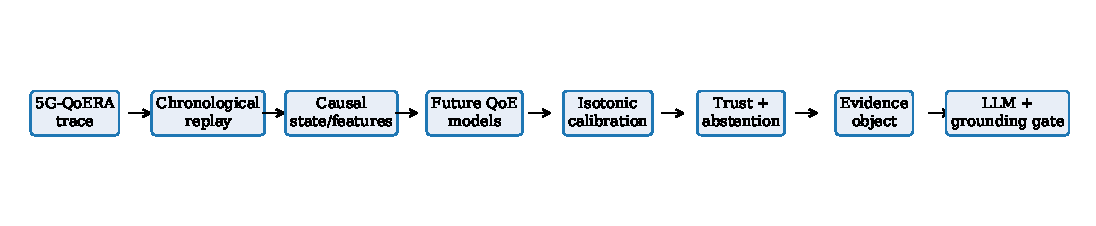
\includegraphics[width=0.98\textwidth]{architecture.pdf}
\caption{Prototype architecture.  The language model is downstream of the
prediction and trust decision and cannot modify either.}
\label{fig:architecture}
\end{figure*}

The twin contains the four mandatory elements:

\begin{enumerate}
\item \textbf{Replay:} rows are globally sorted by timestamp and stable
      session identifier; per-session histories advance only after the
      current row is reached.
\item \textbf{State:} each session stores user, timestamp, base station, PRB,
      latitude, longitude, throughput, bitrate, resolution, packet loss,
      current MOS, session step, and elapsed session time.
\item \textbf{Future event:} the classifier predicts poor QoE at the next
      valid observation in the same session.
\item \textbf{Reliability:} a calibrated probability is accompanied by a
      trust score, level, and abstention decision.
\end{enumerate}

The study is offline and trace-driven.  Observations are correlated and are
not statistically independent.  A row represents one bitrate
alternative attached to a physical radio observation; the prototype studies
\PhysicalObservations physical observations and \SampleSessions reconstructed
sessions rather than claiming that the dataset contains millions of distinct
physical devices.  This distinction matters when interpreting statistical
independence and scale.

\section{Methodology}

\subsection{Dataset Preparation and Sampling}

The upstream repository contains 32 tab-separated scenarios: four base
stations by eight PRB allocations (5 through 40).  The raw wide tables contain
4,147,536 physical rows.  Four configured video alternatives (2,000, 4,000,
6,000, and 8,000~kbps) yield approximately 16.59 million long-format rows.

The frozen experiment uses a resource-safe, earliest-time group-balanced
sample of \SampleRows rows.  It retains complete sessions and covers every
base-station, PRB, and selected-bitrate group.  The sample is authenticated by
SHA-256, checked against all 32 trusted raw files, and then stripped of
inherited session and target fields.  Sessions and labels are reconstructed
from base measurements.  Verification found zero missing source rows, zero value
mismatches in throughput, position, packet loss, or MOS, and zero duplicate row
identities.  After removing \SampleSessions terminal rows and 192 labels that
cross chronological boundaries, \FinalRows labelled rows remain.

\begin{table}[t]
\caption{Chronological dataset partitions}
\label{tab:dataset}
\centering
\resizebox{\columnwidth}{!}{\begin{tabular}{lrrrr}
\toprule
Split & Rows & Sessions & Users & Poor rate \\
\midrule
Train & 537,504 & 51,232 & 216 & 30.18\% \\
Validation & 180,224 & 17,152 & 167 & 37.35\% \\
Test & 179,328 & 18,144 & 181 & 41.43\% \\
\bottomrule
\end{tabular}
}
\end{table}

Table~\ref{tab:dataset} reports the global 60/20/20 time split.  This evaluates
temporal generalization, not generalization to unseen users or cells.  It is
important that the poor-QoE prevalence rises from 30.18\% in training to
41.43\% in test; accuracy alone would therefore hide a meaningful temporal
distribution shift.

\subsection{Session Construction, Horizon, and Target}

A trajectory is grouped by base station, PRB, bitrate, and user.  A new session
begins when the time gap exceeds 30~s.  Within a session, the event is

\begin{equation}
y_t = \mathbb{1}\!\left[\mos_{t+1} < 3.0\right].
\label{eq:target}
\end{equation}

MOS exactly equal to 3.0 is not labelled poor.  The last row of each session
has no future target and is excluded.  Labels whose $t+1$ timestamp crosses a
split boundary are also excluded.  The horizon is one observation, consistent
with the trace sampling process.  It is not a fixed 10-second horizon: the
mean is \MeanLead~s, median \MedianLead~s, and 95th percentile
\PninetyfiveLead~s.  Equation~\ref{eq:target} predicts future poor state, not
the onset of degradation; poor-to-poor transitions are positive events.

\subsection{Causal Feature Contract and Twin State}

Feature generation sorts each session chronologically.  Lag variables use
\texttt{shift}; rolling means and standard deviations shift before rolling, so
the historical window contains only times earlier than $t$.  Current state is
permitted because it is available at the prediction instant.  Future MOS,
future timestamp, target, and retrospective lead time are never model inputs or
LLM evidence.

The network-only contract contains throughput, PRB, base station, position,
time gap, past throughput, movement distance/speed, session step, and elapsed
time.  The cross-layer contract adds bitrate, resolution, current packet loss,
current MOS, lagged and rolling MOS/loss, throughput-to-bitrate ratio, capacity
margin, and an insufficiency flag.  Consequently, the required radio,
mobility, resource-allocation, video, and current-QoE aspects are represented.

Replay parity is tested on interleaved synthetic sessions: the feature vector
computed by online-style replay must equal the batch past-only vector.  A
future-invariance test perturbs later rows and verifies that earlier features
and predictions do not change.  These tests validate the implementation
contract, although they do not replay every one of the \TestRows test rows at
unit-test time.

\subsection{Models}

All learned preprocessing is fitted on training rows only.

\begin{itemize}
\item \textbf{Persistence:} predict future poor QoE when current MOS is below
      3.0.  Its hard 0/1 output supplies a strong temporal baseline.
\item \textbf{Network Logistic Regression:} a balanced, standardized linear
      pipeline receives only the network feature contract.
\item \textbf{Cross-layer Random Forest:} 100 trees, depth 14,
      minimum leaf size 20, 50\% per-tree sampling, and balanced subsampling
      receive the full cross-layer contract; seed 42 fixes stochastic choices.
\end{itemize}

The comparison separates the value of cross-layer state from persistence and
from a network-only linear model.  No test labels are used in fitting,
calibration, or threshold selection.  Final training, calibration, inference,
and evaluation use the same
\texttt{cross\_layer\_random\_forest\_final.joblib} artifact and validate the
complete model $\rightarrow$ calibrator $\rightarrow$ prediction lineage.

\subsection{Calibration and Operating-Point Selection}

The validation period is divided chronologically.  The first 90,208 rows fit
sigmoid and isotonic calibrators.  After removing labels crossing the internal
boundary, the later 89,952 rows select the calibration method by minimum ECE,
then minimum Brier score, then maximum F1.  A fixed threshold grid from 0.05 to
0.95 selects maximum F1, breaking ties by precision.  Table~\ref{tab:cal}
shows the frozen validation choices.  Both learned models selected isotonic
calibration; the Random Forest threshold was \DecisionThreshold.

\begin{table}[t]
\caption{Validation-selected calibration and thresholds}
\label{tab:cal}
\centering
\resizebox{\columnwidth}{!}{\begin{tabular}{lrrrrr}
\toprule
Model & Method & Threshold & F1 & Brier & ECE \\
\midrule
Network Logistic & Isotonic & 0.35 & 0.6670 & 0.1886 & 0.0124 \\
Cross-layer RF & Isotonic & 0.37 & 0.8680 & 0.0741 & 0.0121 \\
\bottomrule
\end{tabular}
}
\end{table}

For test labels $y_i$ and probabilities $p_i$, the Brier score is

\begin{equation}
\mathrm{Brier}=\frac{1}{n}\sum_{i=1}^{n}(p_i-y_i)^2,
\end{equation}

and 10-bin ECE is

\begin{equation}
\ece=\sum_{b=1}^{B}\frac{|S_b|}{n}
\left|\operatorname{acc}(S_b)-\operatorname{conf}(S_b)\right|.
\end{equation}

We additionally report F1, precision, recall, PR-AUC, ROC-AUC, false-positive
count, false-alarm rate $\mathrm{FP}/(\mathrm{FP}+\mathrm{TN})$, and the
observed next-row interval.

\subsection{Trust Score and Abstention}

Let $\tau$ be the selected classification threshold.  Probability confidence
is normalized distance from $\tau$, reaching zero at the boundary and one at
the endpoint on the corresponding decision side.  The YAML-backed score is

\begin{align}
T={}&0.40C_{\tau}(p)+0.30F_{1,\mathrm{val}} \\
   &+0.20(1-\ece_{\mathrm{val}})+0.10Q_{\mathrm{data}}.
\label{eq:trust}
\end{align}

Prediction stability is retained as a diagnostic field but, by design, has no
weight in Equation~\ref{eq:trust}.  The trust score is a ranking heuristic,
not $P(\mathrm{correct})$.  On the later validation half, the abstention
threshold minimizes selective risk subject to at least 90\% coverage.  The
frozen value \TrustThreshold achieves \ValidationCoverage validation coverage and is then
applied unchanged to test.

\subsection{Grounded LLM Component}

The allow list contains decision, calibrated poor-QoE probability, trust score
and level, current MOS, throughput, bitrate, capacity margin,
throughput-to-bitrate ratio, and packet loss.  It excludes labels and all
future-derived fields.  The requested output contains predicted event,
confidence, summary, likely causes with exact evidence keys, operator checks,
and limitations.  For an abstention, confidence must be low, likely causes
must be empty, and the text must say that evidence is insufficient.

Validation occurs in two stages.  A strict Pydantic schema forbids extra or
missing structure.  A deterministic grounding validator checks prediction
polarity, confidence/trust agreement, unsupported numbers, field/value and
unit attribution, cause citations, and abstention behavior.  Failed output is
rejected rather than repaired silently.  The external completion model and
request metadata for the retained offline batch were not preserved, so this
report deliberately makes no provider/model attribution.

\section{Actions Performed and Software Implementation}

The implementation work proceeded through the following actions:

\begin{enumerate}
\item inspected the 32 public scenarios and normalized selected application
      bitrate/MOS columns into long form;
\item authenticated the pinned resource-safe sample and verified every sampled
      base measurement against source TSV bytes;
\item rebuilt sessions, next-row labels, and chronological split boundaries,
      discarding inherited derived fields;
\item implemented past-only features and a per-session replay engine with
      explicit state;
\item trained the three required models and stored model/configuration lineage;
\item fitted sigmoid and isotonic calibration on the first validation half and
      selected calibration, decision, and abstention thresholds on the second;
\item evaluated the frozen models once on the sealed test period;
\item retained and revalidated a repository batch of 30 balanced explanation
      cases (10 accepted poor-QoE, 10 accepted acceptable-QoE, and 10
      abstentions) with completed one-person manual review;
\item added unit, causality, parity, lineage, grounding, and artifact-contract
      tests; and
\item replaced stale publication tables with a generator that checks five
      authoritative result documents before producing this report.
\end{enumerate}

Source modules and scripts include docstrings, type hints, and focused comments
around temporal shifts, split boundaries, trust semantics, evidence allow
lists, and validation rules.  The code is therefore submitted as the required
commented implementation rather than copied into the paper.  The repository's
test suite exercises target generation, chronological splitting, replay,
features, calibration, trust, models, evidence, explanation schema, grounding,
human review, and artifact lineage.

\section{Results}

\subsection{Model Comparison}

Table~\ref{tab:models} evaluates all models on the same \TestRows test rows.
The persistence baseline is strong (F1 0.8403), confirming high temporal
autocorrelation in MOS.  The network-only Logistic Regression underperforms
both alternatives, particularly in false alarms.  The cross-layer Random
Forest achieves the best F1 and PR-AUC and the lowest Brier score and ECE.

\begin{table*}[t]
\caption{Sealed-test comparison; lower Brier, ECE, and false-alarm rate are better}
\label{tab:models}
\centering
\begin{tabular}{lrrrrrr}
\toprule
Model & F1 & PR-AUC & Brier & ECE & FP & FAR \\
\midrule
Persistence & 0.8403 & 0.7719 & 0.1325 & 0.1325 & 11,951 & 11.38\% \\
Network Logistic & 0.6784 & 0.6459 & 0.1941 & 0.0216 & 45,512 & 43.33\% \\
Cross-layer RF & 0.8807 & 0.9549 & 0.0715 & 0.0116 & 8,365 & 7.96\% \\
\bottomrule
\end{tabular}

\end{table*}

\begin{figure*}[t]
\centering
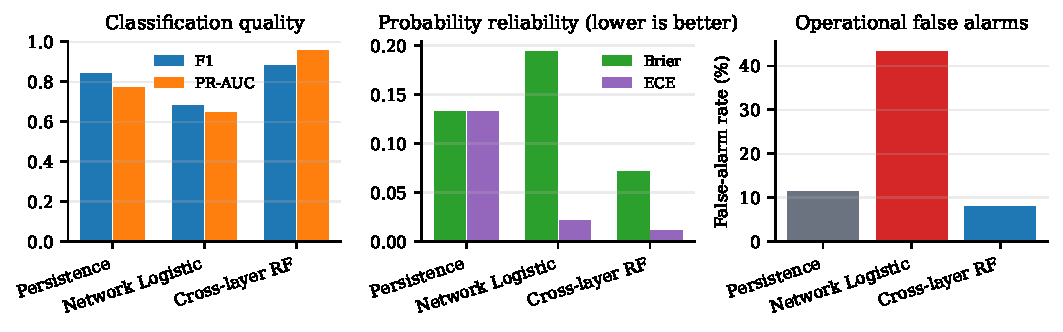
\includegraphics[width=0.98\textwidth]{model_comparison.pdf}
\caption{Classification, probability-reliability, and false-alarm comparison
on the sealed test period.}
\label{fig:models}
\end{figure*}

The final Random Forest yields accuracy \RFAccuracy, precision \RFPrecision,
recall \RFRecall, F1 \RFFone, PR-AUC \RFPRAUC, ROC-AUC \RFROCAUC, Brier
\RFBrier, and ECE \RFECE.  Its confusion matrix contains \TrueNegatives true negatives,
\FalsePositives false positives, \FalseNegatives false negatives, and \TruePositives true
positives.  Thus the false-alarm rate is \FalseAlarmRate and the miss rate is
\MissRate.  Reporting both counts and rates avoids hiding the operational burden
created by a large test set.

The model comparison supports the cross-layer hypothesis.  The Random Forest
improves F1 by \FoneVsPersistence over persistence and by \FoneVsNetwork over network-only Logistic
Regression.  Its PR-AUC exceeds persistence by \PRAUCVsPersistence and the network-only
model by \PRAUCVsNetwork.  Because the test positive rate is \TestPoorRate, PR-AUC is
more informative than accuracy alone.

\subsection{Calibration and the Research Question}

Low ECE and Brier error show that the best classifier is also well calibrated
in aggregate on this chronological test period.  This is not automatic: the
network-only model has ECE 0.0216 but poor F1 0.6784, whereas persistence has
strong F1 but ECE 0.1325 because its binary scores are overconfident.
Discrimination and calibration must therefore be measured separately.  The
cross-layer Random Forest is the only model that combines high PR-AUC with low
Brier and ECE.

The answer to the main research question is consequently \emph{yes for the
frozen 5G-QoERA time period}: the best classification model is sufficiently
calibrated to support a selective operator policy.  The answer is not a claim
of universal reliability; ECE is aggregate and later sections identify drift,
sampling, and external-validity limits.

\subsection{Trust, Coverage, and Selective Accuracy}

Applying the validation-selected threshold abstains on \AbstainedCount of
\TestRows rows (\AbstentionRate) and covers \Coverage.  Table~\ref{tab:final}
and Figure~\ref{fig:selective} show the resulting trade-off.  Accepted accuracy
rises from \RFAccuracy to \AcceptedAccuracy; accepted precision is
\AcceptedPrecision, recall \AcceptedRecall, and F1 \AcceptedFone.  Accepted
Brier score and ECE also improve to \AcceptedBrier and \AcceptedECE.

\begin{table}[t]
\caption{Overall versus accepted test decisions}
\label{tab:final}
\centering
\resizebox{\columnwidth}{!}{\begin{tabular}{lrrrrrr}
\toprule
Scope & Acc. & Prec. & Recall & F1 & Brier & ECE \\
\midrule
All predictions & 0.9018 & 0.8860 & 0.8755 & 0.8807 & 0.0715 & 0.0116 \\
Accepted only & 0.9340 & 0.9299 & 0.9091 & 0.9194 & 0.0542 & 0.0090 \\
\bottomrule
\end{tabular}
}
\end{table}

\begin{figure}[t]
\centering
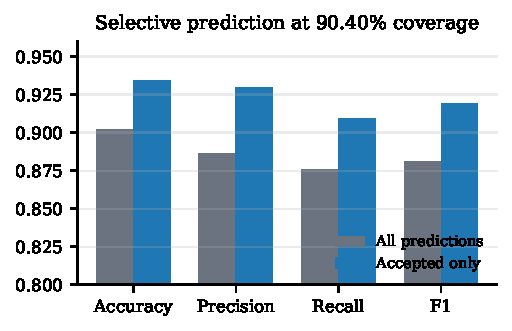
\includegraphics[width=\columnwidth]{selective_performance.pdf}
\caption{Abstention improves accepted-decision performance while retaining
\Coverage coverage.}
\label{fig:selective}
\end{figure}

This improvement is descriptive, not a second test-tuned operating point: the
trust policy and threshold were fixed entirely on validation data.  Coverage
remains above the 90\% constraint.  An operator can interpret an accepted
high/medium-trust decision as eligible for support, while an abstention means
``collect or verify more evidence,'' not ``acceptable QoE.''

\subsection{Cross-Layer Drivers}

Figure~\ref{fig:importance} ranks the leading impurity-based Random Forest
features.  Packet-loss percentage and throughput-to-bitrate ratio dominate,
followed by capacity margin, capacity insufficiency, and current MOS.  Past MOS
and loss variables also contribute.  This pattern is consistent with the
research design: future experience depends on delivery capacity relative to
application demand and on recent service state, not on throughput in
isolation.  Importance is associative and global; it does not prove a causal
network fault for an individual event.

\begin{figure}[t]
\centering
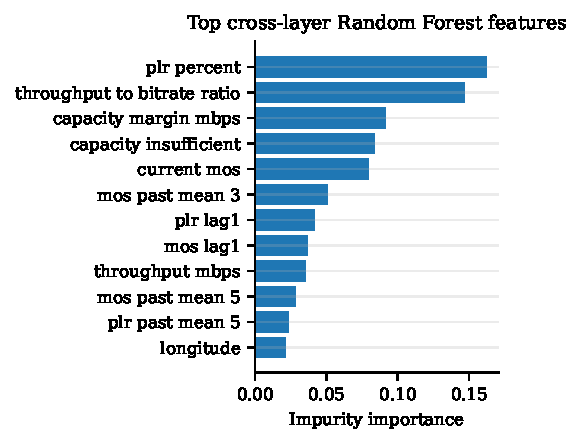
\includegraphics[width=\columnwidth]{feature_importance.pdf}
\caption{Top twelve cross-layer Random Forest features.}
\label{fig:importance}
\end{figure}

\subsection{Prediction Horizon}

Figure~\ref{fig:lead} summarizes the actual one-step interval.  Most rows are
near 10~s, but the range extends from roughly zero to 30~s.  The median
\MedianLead~s provides a short investigation window for an edge operator, yet
it should not be reported as guaranteed ``lead time before onset.''  The target
is next-state poor QoE, and the dataset does not label a unique degradation
onset.

\begin{figure}[t]
\centering
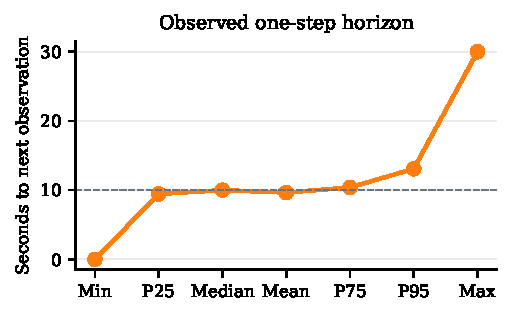
\includegraphics[width=\columnwidth]{lead_time_summary.pdf}
\caption{Observed time from each prediction row to its next in-session row.}
\label{fig:lead}
\end{figure}

\section{Explanation Evaluation}

The balanced 30-case batch contains the three operational outcomes needed to
exercise the interface.  Table~\ref{tab:llm} and Figure~\ref{fig:llm} report
the retained evaluation.  All outputs parse under the strict schema and pass
the grounding validator.  The single reviewer judged all 30 factually correct
and complete, with zero unsupported-statement and contradiction flags.

\begin{table}[t]
\caption{Grounded explanation evaluation}
\label{tab:llm}
\centering
\begin{tabular}{lr}
\toprule
Measure & Result \\
\midrule
Retained/reviewed & 30/30 \\
Schema valid & 30 (100\%) \\
Grounding valid & 30 (100\%) \\
Factual and complete & 30 (100\%) \\
Unsupported statements & 0 (0\%) \\
Contradictions & 0 (0\%) \\
\bottomrule
\end{tabular}

\end{table}

\begin{figure}[t]
\centering
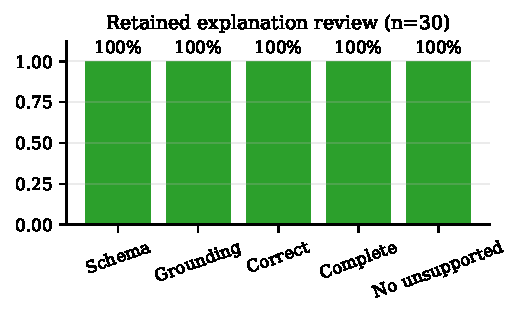
\includegraphics[width=\columnwidth]{llm_validation.pdf}
\caption{Validation and manual-review outcomes for the retained explanation
batch.}
\label{fig:llm}
\end{figure}

A typical accepted poor-QoE explanation reports the future event and confidence,
then associates a negative capacity margin and packet loss with the forecast,
citing the corresponding keys.  It tells the operator to verify throughput
against bitrate, inspect packet loss, and confirm whether current MOS conditions
persist.  It also states that evidence does not identify a unique root cause.
For an abstention, the explanation makes no causal diagnosis and recommends
collecting another observation.  This satisfies the requirement to explain
the event, likely causes, confidence/limitations, and operator checks while
preventing invented numeric values.

The 100\% rates must be interpreted cautiously.  The set is small, deliberately
balanced rather than prevalence weighted, reviewed by one person, and based on
externally completed outputs whose provider/model metadata were not retained.
The result demonstrates a working grounded interface, not population-wide LLM
quality or inter-rater reliability.

\section{Discussion}

Three findings matter for trustworthy management.  First, persistence is a
demanding baseline.  A future-QoE paper that omitted it could mistake temporal
autocorrelation for model intelligence.  The cross-layer model nevertheless
adds measurable value in F1, PR-AUC, and false alarms.

Second, classification and calibration can disagree.  Network-only Logistic
Regression is relatively calibrated yet not sufficiently discriminative at
the chosen operating point; persistence classifies well but supplies poor
probabilities.  The calibrated cross-layer Random Forest performs well on both
dimensions.  This directly answers the study's central question and justifies
reporting F1, PR-AUC, Brier, and ECE together.

Third, a single probability does not complete a trustworthy interface.  The
validation-selected reject option improves the accuracy of decisions offered
to an operator and explicitly routes ambiguous cases to further verification.
The explanation layer then makes evidence and limitations visible without
controlling the predictor.  This separation of authority is valuable: model
output, reliability policy, and language generation can each fail independently
and are validated at their boundaries.

The project also illustrates scale honestly.  Millions of modelling rows and
tens of thousands of sessions exercise distributed trace processing, but they
do not constitute millions of independent physical Things.  Four bitrate
alternatives share each physical radio observation, and repeated rows from a
user/session are correlated.  The prototype addresses the assignment's
large-scale management context without inflating its empirical unit count.

\section{Limitations and Threats to Validity}

\textbf{Offline scope:} trace replay approximates online evolution but cannot
reproduce feedback between a control action and future radio conditions.  No
closed-loop resource change is executed.

\textbf{Sampling and provenance:} the final experiment uses a pinned,
earliest-time group-balanced sample rather than the complete 16.59-million-row
long table.  Raw compatibility and byte identity are strong, but the historical
command that produced the sample is unavailable.  It should therefore remain
labelled a quarantined external snapshot.  The result is scientifically
traceable but not fully regenerable from the public raw data alone without a
new declared sampling policy and new results.

\textbf{Dependence and generalization:} bitrate alternatives share radio
observations, and sessions/users may recur across periods.  A global time split
tests later-time performance, not unseen-user, unseen-cell, or unseen-city
performance.  Results may not transfer to other codecs, services, deployments,
or traffic regimes.

\textbf{Target construct:} MOS below 3.0 is an explicit, reproducible poor-state
definition, but other thresholds or onset-only targets would change prevalence
and action meaning.  The one-step interval is irregular and short.

\textbf{Calibration:} ECE depends on binning and aggregate test performance can
hide subgroup miscalibration.  Isotonic mappings may require recalibration
under drift.  The trust equation is a policy heuristic; its weights were not
learned from measured operational cost.

\textbf{Interpretation:} impurity importance and LLM likely-cause statements
express supported associations, not causality.  Automatic grounding focuses on
structured fields, values, units, and obvious contradictions; it cannot prove
that every non-numeric semantic implication is warranted.

\textbf{Explanation evaluation:} 30 cases and one reviewer do not establish
inter-rater reliability.  Missing external completion metadata also limits
exact generation reproducibility, even though the retained outputs, prompts,
schemas, validations, and human judgments are preserved.

\section{Suggestions for Improvement}

The following actions would materially strengthen the work:

\begin{enumerate}
\item publish a deterministic sample builder or rerun the full dataset on
      higher-memory infrastructure, recording data, configuration, code, model,
      and result hashes in one run manifest;
\item evaluate rolling-origin and blocked cross-validation, plus held-out users,
      cells, and scenario files, to separate temporal from entity
      generalization;
\item compare onset-specific, fixed-time, and multi-horizon targets and report
      event-based warning lead time rather than only the next-row interval;
\item add subgroup reliability diagrams, adaptive/calibration error variants,
      class-conditional calibration, bootstrap confidence intervals, and drift
      monitoring;
\item choose trust and decision thresholds from explicit false-alarm, miss,
      abstention, and intervention costs, then validate the policy prospectively;
\item compare calibrated Gradient Boosting and temporal models under the same
      leakage-safe protocol, with ablations for application, mobility, and
      historical QoE feature families;
\item extend the twin to streaming ingestion and counterfactual ``what-if''
      resource-allocation experiments, while keeping the LLM outside the
      control loop;
\item strengthen grounding with semantic entailment checks, unit ontologies,
      allow-listed causal templates, adversarial prompts, and rejection tests;
      and
\item retain provider/model/version/request metadata and conduct blinded review
      with multiple network-domain operators, reporting inter-rater agreement
      and usefulness/actionability scores.
\end{enumerate}

\section{Conclusion}

This work delivers the requested small, scientifically valid 5G QoE Digital
Twin.  It chronologically replays the public 5G-QoERA trace, maintains a
cross-layer state, forecasts next-observation poor QoE, calibrates its best
model, quantifies trust and abstention, and produces evidence-grounded operator
explanations.  The calibrated Random Forest achieves F1 \RFFone, PR-AUC
\RFPRAUC, Brier \RFBrier, and ECE \RFECE on \TestRows later-time rows.
Selective abstention preserves \Coverage coverage while raising accepted
accuracy to \AcceptedAccuracy.  The 30 retained explanations pass automated
and manual factuality checks without unsupported values.

The central conclusion is nuanced: good cross-layer classification and good
aggregate calibration do coexist here, and a validation-selected reject option
improves the reliability of operator-facing decisions.  The prototype remains
an offline research twin, not a commercial system.  Full raw-data
reproducibility, external scenario validation, cost-based trust design, drift
monitoring, semantic grounding, and multi-reviewer explanation studies are the
most important next steps.

\section*{Acknowledgment}
This project was conducted in the PGE 5 Artificial Intelligence and Data
Science program at Aivancity School for Technology, Business \& Society.

\bibliographystyle{IEEEtran}
\bibliography{references/references}

\end{document}
